% В этом документе преамбула

%%% Работа с русским языком
\usepackage{cmap}					% поиск в PDF
\usepackage{mathtext} 				% русские буквы в формулах
\usepackage[T2A]{fontenc}			% кодировка
\usepackage[utf8]{inputenc}			% кодировка исходного текста
\usepackage[english,russian]{babel}	% локализация и переносы
\usepackage{indentfirst}			% чтобы первый абзац в разделе отбивался красной строкой
\frenchspacing						% тонкая настройка пробелов

%%% Приведение начертания букв и знаков к русской типографской традиции
\renewcommand{\epsilon}{\ensuremath{\varepsilon}}
\renewcommand{\phi}{\ensuremath{\varphi}}			% буквы "эпсилон"
\renewcommand{\kappa}{\ensuremath{\varkappa}}		% буквы "каппа"
\renewcommand{\le}{\ensuremath{\leqslant}}			% знак меньше или равно
\renewcommand{\leq}{\ensuremath{\leqslant}}			% знак меньше или равно
\renewcommand{\ge}{\ensuremath{\geqslant}}			% знак больше или равно
\renewcommand{\geq}{\ensuremath{\geqslant}}			% знак больше или равно
\renewcommand{\emptyset}{\varnothing}				% знак пустого множества

%%% Дополнительная работа с математикой
\usepackage{amsmath,amsfonts,amssymb,amsthm,mathtools} % AMS
\usepackage{icomma} % "Умная" запятая: $0,2$ --- число, $0, 2$ --- перечисление

%% Номера формул
\mathtoolsset{showonlyrefs=true} % Показывать номера только у тех формул, на которые есть \eqref{} в тексте.

%% Свои команды

% операции, не определённые (или имеющие иные обохначения) в мат. пакетах
\DeclareMathOperator{\sgn}{\mathop{sgn}}				% ф-ия sgn
\renewcommand{\tg}{\mathop{\mathrm{tg}}\nolimits}		% обозначение тангенса

%% Перенос знаков в формулах (по Львовскому)
\newcommand*{\hm}[1]{#1\nobreak\discretionary{}
{\hbox{$\mathsurround=0pt #1$}}{}}

%%% Работа с картинками
\usepackage{graphicx}  % Для вставки рисунков
\graphicspath{{images/}{images2/}}  % папки с картинками
\setlength\fboxsep{3pt} % Отступ рамки \fbox{} от рисунка
\setlength\fboxrule{1pt} % Толщина линий рамки \fbox{}
\usepackage{wrapfig} % Обтекание рисунков текстом

%%% Работа с таблицами
\usepackage{array,tabularx,tabulary,booktabs} % Дополнительная работа с таблицами
\usepackage{longtable}  % Длинные таблицы
\usepackage{multirow} % Слияние строк в таблице

%%% Теоремы
\theoremstyle{plain} % Это стиль по умолчанию, его можно не переопределять.
\newtheorem{theorem}{Теорема}[section]
\newtheorem{lemma}{Лемма}[section]
\newtheorem{definition}[theorem]{Определение}
\newtheorem{property}{Свойство}
 
\theoremstyle{definition} % "Определение"
\newtheorem{corollary}{Следствие}[theorem]
\newtheorem{exmp}{Пример}[section]
 
\theoremstyle{remark} % "Примечание"
\newtheorem*{nonum}{Решение}
\newtheorem*{evidence}{Доказательство}
\newtheorem*{remark}{Примечание}

%%% Программирование
\usepackage{etoolbox} % логические операторы

%%% Страница
\usepackage{extsizes} % Возможность сделать 14-й шрифт
\usepackage{geometry} % Простой способ задавать поля
	\geometry{top=25mm}
	\geometry{bottom=35mm}
	\geometry{left=35mm}
	\geometry{right=20mm}

%\usepackage{fancyhdr} % Колонтитулы
% 	\pagestyle{fancy}
 	%\renewcommand{\headrulewidth}{0pt}  % Толщина линейки, отчеркивающей верхний колонтитул
% 	\lfoot{Нижний левый}
% 	\rfoot{Нижний правый}
% 	\rhead{Верхний правый}
% 	\chead{Верхний в центре}
% 	\lhead{Верхний левый}
%	\cfoot{Нижний в центре} % По умолчанию здесь номер страницы

\usepackage{setspace} % Интерлиньяж (межстрочные интервалы)
%\onehalfspacing % Интерлиньяж 1.5
%\doublespacing % Интерлиньяж 2
%\singlespacing % Интерлиньяж 1

\usepackage{lastpage} % Узнать, сколько всего страниц в документе.

\usepackage{soulutf8} % Модификаторы начертания

\usepackage{hyperref}
\usepackage[usenames,dvipsnames,svgnames,table,rgb]{xcolor}
\hypersetup{				% Гиперссылки
    unicode=true,           % русские буквы в раздела PDF
    pdftitle={Заголовок},   % Заголовок
    pdfauthor={Автор},      % Автор
    pdfsubject={Тема},      % Тема
    pdfcreator={Создатель}, % Создатель
    pdfproducer={Производитель}, % Производитель
    pdfkeywords={keyword1} {key2} {key3}, % Ключевые слова
    colorlinks=true,       	% false: ссылки в рамках; true: цветные ссылки
    linkcolor=MidnightBlue,          % внутренние ссылки
    citecolor=black,        % на библиографию
    filecolor=magenta,      % на файлы
    urlcolor=blue           % на URL
}

\usepackage{csquotes} % Еще инструменты для ссылок

%\usepackage[style=authoryear,maxcitenames=2,backend=biber,sorting=nty]{biblatex}

\usepackage{multicol} % Несколько колонок

%%% Работа с графикой
\usepackage{tikz}
\usetikzlibrary{calc}
\usepackage{tkz-euclide}
\usetikzlibrary{arrows}
\usepackage{pgfplots}
\usepackage{pgfplotstable}

%%% Настройка подписей к плавающим объектам
\usepackage{floatrow}	% размещение
\usepackage{caption}	% начертание
\captionsetup[figure]{labelfont=bf,textfont=it,font=footnotesize}	% нумерация и надпись курсивом
% для подфигур: заголовок подписи полужирный, текст заголовка обычный
% выравнивание является неровным (т.е. выровненным по левому краю)
% singlelinecheck = off означает, что настройка выравнивания используется, даже если заголовок имеет длину только одну строку.
% если singlelinecheck = on, то заголовок всегда центрируется, когда заголовок состоит только из одной строки.
\captionsetup[subfigure]{labelfont=bf,textfont=normalfont,singlelinecheck=off,justification=raggedright}

%%% Stuff для графиков и рисунков



\begin{document}

Белые и чёрные шары распределены по ящикам следующим образом:

\begin{figure}[H]
	\center{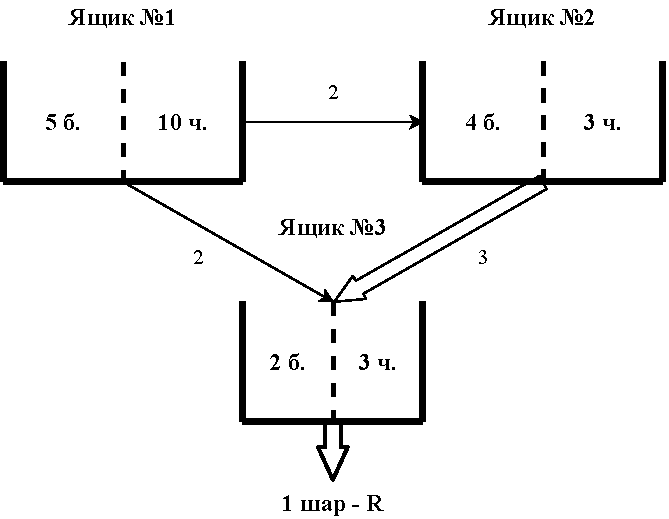
\includegraphics[scale=1]{../media/Homework-29-02-20_2.pdf}}
\end{figure}

\textit{Решение:}

Отслеживаем, как белые шары двигались по ящикам.

\begin{itemize}
	\item Событие $A$ - вытащен белый шар. 
	\item Событие $H_i$ - вытащенный шар изначально был в $i$-ом ящике, $i=1,2,3$.
	\item Событие $B_j$ - вытащенный из 3-его ящика шар пришёл в него из $j$-ого ящика, $j=1,2,3$.
\end{itemize}

Всего в 3-ем ящике по итогу 10 шаров.

\begin{figure}[H]
	\center{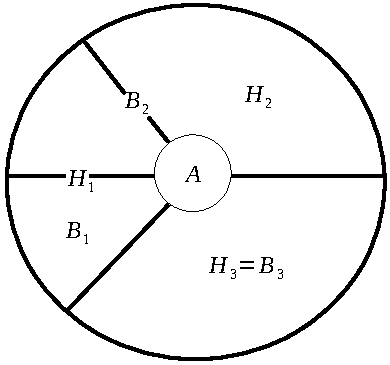
\includegraphics[scale=1]{../media/Homework-29-02-20_3.pdf}}
\end{figure}

\begin{remark}
	$B_2$ находится между $H_1$ и $H_2$, т.к. из 2-ого ящика мы можем достать шар, который изначально в нём содержался, либо же тот, что пришёл в него из 1-ого.
\end{remark}

\begin{table}[h]
	\centering
	\begin{tabular}{|c|c|c|}
		2 шара из 1-ого ящ. & 3 шара из 2-ого ящ. & 5 шаров было в 3-ем \\ \hline
	\end{tabular}
	\caption*{Содержание 3-его ящика}
\end{table}

Рассмотрим вероятности достать белый шар, в зависимости от того, где он первоначально находился:

\begin{table}[H]
	\centering\makegapedcells
	\begin{tabular}{|c|c|c|c|}
		\hline
		$i$        & 1             & 2             & 3              \\ \hline
		$P(H_i)$   & $?$           & $?$           & $\frac{5}{10}$ \\ \hline
		$P(A|H_i)$ & $\frac{5}{10+5}=\frac{1}{3}$ & $\frac{4}{4+3}=\frac{4}{7}$ & $\frac{2}{2+3}=\frac{2}{5}$  \\ \hline
	\end{tabular}
\end{table}

\begin{table}[H]
	\centering\makegapedcells
	\begin{tabular}{|c|c|c|c|}
		\hline
		$j$      & 1              & 2              & 3              \\ \hline
		$P(B_j)$ & $\frac{2}{10}$ & $\frac{3}{10}$ & $\frac{5}{10}$ \\ \hline
	\end{tabular}
\end{table}

Очевидно, что вероятность $P(H_3)$ известна, т.к. есть общее количество шаров в 3-ем ящике и изначальное кол-во белых в нём.

Вероятность совместного появления двух зависимых событий равна произведению вероятности одного события на условную вероятность другого события (см. круг):
\[ P(H_1) = P(B_1H_1) + P(B_2H_1) = P(H_1|B_1)P(B_1) + P(H_1|B_2)P(B_2) = \underset{=1}{P(H_1|B_1)} \underset{=\frac{2}{10}}{P(B_1)} + \underset{=\frac{2}{9}}{P(H_1|B_2)} \underset{=\frac{3}{10}}{P(B_2)} \]
\[ P(H_1) = \frac{2}{10} + \frac{2}{9} \cdot \frac{3}{10} = \frac{8}{30} \]

\[ P(H_2) = P(H_2|B_2) P(B_2) = \frac{7}{9} \cdot \frac{3}{10} = \frac{7}{30} \]

\begin{remark}
	$P(H_1|B_1)=1$, т.к. вероятность, что вытащенный шар был изначально в 1-м ящике при условии, что вытащенный из 3-его ящика шар пришёл из 1-ого, очевидно, является тривиальным. $P(H_1|B_2)=\dfrac{2}{9}$ т.к.  во втором ящике $4+3+2$ всего шаров и максимум 2 их них пришли в него из 1-ого. $P(H_2|B_2)=\dfrac{7}{9}$ по тем же причинам - изначально там было 7 шаров.
\end{remark}

В результате для первой строки нашей таблицы получаем:

\[ \frac{8}{30} + \frac{7}{30} + \underset{=\frac{15}{30}}{\frac{5}{10}} = 1 \]
Т.е. всё верно и вычисления 3-ей величины мы производили для проверки. 

\end{document} 